\documentclass[../main.tex]{subfiles}

\begin{document} %%%%%%%%%%%%%%%%%%%%%%%%%%%%%%%%%%%%%%%%%%%%%%%%%%%%%%%%%%%%
\section{Introducción a probabilidad y estadística}
    \subsection{Esperanza}
        \begin{definition}\textbf{(variable discreta)}
            Sea $X$ una variable discreta con función de probabilidad $P_X(x)$. La esperanza de $X$, denotada por $E[X]$, se define por
            \begin{equation}
                E[X] = \sum_{i=1}^{n} x_i \cdot P(X=x_i)
            \end{equation}
        \end{definition}

        \begin{definition}\textbf{(variable absolutamente continua)}
            Sea $X$ una variable absolutamente continua con función de densidad $f_X(x)$. La esperanza de $X$, denotada por $E[X]$, se define por
            \begin{equation}
                E[X] = \int_{-\infty}^{\infty} x \cdot f_X(x) \cdot dx
            \end{equation}
        \end{definition}

    \subsection{Varianza}
        La varianza da una medida de cuánto varían los valores de una muestra obtenida al realizar experimentos aleatorios.

        Los $x_i$ son los valores obtenidos. Mientras que $\bar{X}$ es el promedio de los resultados del experimento. $N$ es la cantidad de resultados obtenidos. \textit{Video Youtube min 5:40} \cite{lista_intro_data_science}

        \begin{equation}
            Var(X) = \frac{1}{N} \cdot \sum_{i=1}^{N} (x_i - \bar{X})^2
        \end{equation}
        
        Cuandio la varianza es baja, los valores de la muestra se agrupn cerca de su valor esperado. Cuando la varianza es alta, los valores de la muestra se dispersan más.

        \begin{definition}(Varianza).
            Sea $X$ una variable aleatoria con esperanza finita. La varianza de $X$ se define por
            \begin{equation}
                 Var(X) = E[(X - E[X])^2]
            \end{equation}
        \end{definition}

        \begin{definition}(Desviación estándar).
            La desviación estándar de $X$ se define por
            \begin{equation}
                \sigma_X = \sqrt{Var(X)}
            \end{equation}
        \end{definition}

    \subsection{Covarianza}
        \begin{definition}\textbf{(Covarianza)}
            La covarianza es una medida de cómo varían conjuntamente dos variables aleatorias.

            Sean $X$ e $Y$ dos variables aleatorias de varianzas finitas definidas sobre el mismo espacio de probabilidad $(\Omega ,A, P)$. La covarianza de $X$ e $Y$ se define por
            \begin{equation}
                \begin{split}
                    Cov(X,Y) &= E[(X - E[X])(Y - E[Y])] 
                    \\&= E[XY] - E[X]E[Y]
                \end{split}
            \end{equation}

            \underline{Interpretación de la covarianza:}
            \begin{itemize}
                \item Si $S_{xy} > 0$ hay dependencia directa (positiva), es decir, a grandes valores de $X$ corresponden grandes valores de $Y$.
                \item Si $S_{xy} < 0$ hay dependencia inversa (negativa), es decir, a grandes valores de $X$ corresponden pequeños valores de $Y$.
                \item Si $S_{xy} = 0$ no hay dependencia lineal entre $X$ e $Y$.
            \end{itemize}
    
            % cargamos imagen
            \begin{figure}[htb]
                \centering
                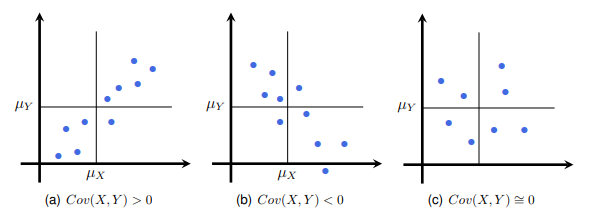
\includegraphics[scale=0.5]{./images/covarianza.png}
                \caption{Covarianza}
                \label{fig:covarianza}
            \end{figure}
            
        \end{definition}

        \begin{definition} \textbf{(Covarianza muestral)} 
            \begin{equation}
                S_{xy} = \frac{1}{n-1} \cdot \sum_{i=1}^{n}(x_i - \bar{x})(y_i - \bar{y})
            \end{equation}

            \begin{equation}
                \bar{x} = \frac{1}{n} \cdot \sum_{i=1}^{n} x_i \quad  \quad \quad \bar{y} = \frac{1}{n} \cdot \sum_{i=1}^{n} y_i
            \end{equation}
        \end{definition}
        
    \subsection{Correlación}
        Es una medida de relación lineal entre dos variables cualitativas continuas. Con esta medida, se logra determinar si las variables varían conjuntamente. \\

        Es una medida normalizada, su valor va de -1 a 1. El caso en el que la correlación es 0, indica que no existe relación lineal entre las variables.

        En caso de que se 1, se trata de correlación perfecta en sentido positivo. En caso de que sea -1, se trata de correlación perfecta en sentido negativo.

        El sentido positivo, indica que varían en el mismo sentido. El sentido negativo, indica que varían en sentidos opuestos.

        \begin{definition} \textbf{(Coeficiente de correlación)}
            \begin{equation}
                \rho(X,Y) = \frac{Cov(X,Y)}{\sigma_X \cdot \sigma_Y}
            \end{equation}
            
        \end{definition}

        \begin{definition} \textbf{(Coeficiente de Correlación de Pearson)}
            \begin{equation}
                \begin{split}
                    \rho_{xy} &= \frac{S_{xy}}{S_x \cdot S_y}
                    \\&= \frac{\sum_{i=1}^{n} (x_i - \bar{x}) \cdot (y_i - \bar{y})}{\sum_{i=1}^{n} (x_i - \bar{x})^2 \cdot \sum_{i=1}^{n} (y_i - \bar{y})^2}
                \end{split}
            \end{equation}

            % cargamos imagen
            \begin{figure}[h]
                \centering
                \includegraphics[scale=0.4]{./images/coeficiente_correlación.png}
                \caption{Coeficiente de Correlación de Pearson}
                \label{fig:coeficiente_correlación}
            \end{figure}
        \end{definition}

        Que las variables esten corelacionadas no implica que haya una relación de causalidad entre las mismas. Por ejemplo, si se toma la temperatura y la cantidad de helados vendidos, ambas variables están correlacionadas, pero no hay una relación de causalidad.

    \subsection{Ejemplos}
        \begin{example}
            Ejemplo de como calcular datos variables aleatorias. Video Youtube \cite{ejemplo_variables_aleatorias}

            \begin{table}[h]
                \centering
                \begin{tabular}{|c|c|}
                \hline
                \textbf{X} & \textbf{Y} \\ \hline
                2          & 1          \\ \hline
                3          & 2          \\ \hline
                5          & 2          \\ \hline
                6          & 3          \\ \hline
                \end{tabular}
                \caption{Datos}
            \end{table}

            \begin{itemize}
                \item \textbf{Esperanza}
                    \begin{equation}
                        \begin{split}
                            E[X] &= \frac{1}{4} \cdot (2 + 3 + 5 + 6) = 4
                            \\E[Y] &= \frac{1}{4} \cdot (1 + 2 + 2 + 3) = 2
                        \end{split}
                    \end{equation}
                \item \textbf{Varianza}
                    \begin{equation}
                        \begin{split}
                            Var(X) &= \frac{1}{4} \cdot [(2 - 4)^2 + (3 - 4)^2 + (5 - 4)^2 + (6 - 4)^2] = 2.5
                            \\Var(Y) &= \frac{1}{4} \cdot ((1 - 2)^2 + (2 - 2)^2 + (2 - 2)^2 + (3 - 2)^2) = 0.5
                        \end{split}
                    \end{equation}
                \item \textbf{Covarianza}
                    \begin{equation}
                        \begin{split}
                            Cov(X,Y) &= \frac{1}{4} \cdot [(2 - 4)(1 - 2) + (3 - 4)(2 - 2) \\
                            &+ (5 - 4)(2 - 2) + (6 - 4)(3 - 2)] \\
                            &= \frac{1}{4} \cdot (2 + 0 + 0 + 2) \\
                            &= 1
                        \end{split}
                    \end{equation}
                
                \item \textbf{Correlación}
                    \begin{equation}
                        \begin{split}
                            \rho_{xy} &= \frac{Cov(X,Y)}{\sigma_X \cdot \sigma_Y} \\
                            &= \frac{1}{\sqrt{2.5} \cdot \sqrt{0.5}} \\
                            &= \sqrt{\frac{4}{5}} = 0.8944
                        \end{split}
                    \end{equation}
            \end{itemize}
        \end{example}


        
\end{document}  %%%%%%%%%%%%%%%%%%%%%%%%%%%%%%%%%%%%%%%%%%%%%%%%%%%%%%%%%%%%%